%  Created by Alexis on 2012-11-04.
%  Copyright (c) 2012 . All rights reserved.
%
%\documentclass[]{article}
%\documentclass[12pt,pdftex,twocolumn]{article}
\documentclass[12pt,pdftex]{article}
% Use utf-8 encoding for foreign characters
\usepackage[utf8]{inputenc}
% Setup for fullpage use
\usepackage{fullpage}
% Surround parts of graphics with box
\usepackage{boxedminipage}
% Package for including code in the document
\usepackage{listings}
% If you want to generate a toc for each chapter (use with book)
%\usepackage{minitoc}
% This is now the recommended way for checking for PDFLaTeX:
\usepackage{ifpdf}

\ifpdf
\usepackage[pdftex]{graphicx}
\else
\usepackage{graphicx}
\fi

\title{CS760 \\ All In \\ Project Report }
\author{  Alexis Fisher }
%\date{2012-11-04}
\begin{document}
\ifpdf
\DeclareGraphicsExtensions{.pdf, .jpg, .tif}
\else
\DeclareGraphicsExtensions{.eps, .jpg}
\fi
\maketitle
\begin{abstract}
\emph{All In} is a five card draw poker player.  
The implemented player uses reinforcement learning to outperform a random player. 
The learner has imperfect knowledge of the opposing player.
The implemented learner performs better than the random player, winning more than 60\% of games played.

%Intro approach evaluation discussion conclusion
\end{abstract}
\section{Introduction}
%Introduction: what you attempted to do, and what the motivation is.
\emph{All In} implements a 5-card draw poker player. The primary goal of the \emph{All In} player is to outperform a random player. Initial implementation assumes two players. The players consist of the learned player and another player. The other player can be either random, a person, or another learned player. 

\section{Approach}
\begin{table*}[ht]
\centering
	\begin{tabular}{| r | r | l |}
\hline
\textbf{Value} & \textbf{Name} & \textbf{Description} \\
\hline
0 & high card & No other match \\
1 & one pair & Single pair of a single value\\
2 & two pairs & Two pairs of distinct values\\
3 & three of a kind & Three cards of a single value\\
4 & straight & Sequentially numbered cards\\
5 & flush & All cards of a single suit\\
6 & full house & Distinct three of a kind and pair\\
7 & four of a kind & Four cards of a single value\\
8 & straight flush & Sequential numbered cards of a single suit\\
9 & royal flush & Straight flush with an Ace as high card\\
\hline
\end{tabular}
\caption{Description of Values according to hand}
\label{tab:cardvalues}
\end{table*}

\emph{All In} uses nondeterministic \emph{Q} reinforcement learning, with a value function determined by the hand's rank and past performance (Wins or Losses). This value is described in Table \ref{tab:cardvalues}. 
Because results of a given hand are nondeterministic, exploration happens organically. 
Win/Loss probability uses Laplace smoothing to account for values the learner has not yet encountered. This is pessimistic- if the learner achieves a royal flush, there is a much higher likelihood of winning than the 50\% indicated in Table \ref{tab:rand_val_res}. 

As the rules of poker vary wildly, a quick description of the rules is appropriate.
Each player is dealt a hand of five cards from a standard 52 card deck. 
Each player has the opportunity to discard up to three cards, and receive replacements from the deck.
Poker hands as described in Table \ref{tab:cardvalues} are used to determine the winner.
%Approach: what you did. If you developed your own approach, you should describe your work in sufficient detail that someone else could replicate your work. If you are using previously developed algorithms, describe them briefly, and provide references to complete descriptions. Don't describe your code organization or implementation details. For the intended audience, you should assume that interested readers could figure out how to implement the code as long as the algorithm is described in sufficient detail.

%To create a 5-card draw poker player implemented via a reinforcement-learning approach.  The constructed Player will retain memory of its initial and current hand to decide which cards to forfeit during the draw. To learn the Q algorithm, the reward signal is the ranking of the player's current poker hand, and the actions available are drawing [0-3] cards. I plan to implement this in Python.

\section{Evaluation}

%Empirical Evaluation: describe your experiments and results. Describe your data sets in adequate detail. If you selected a subset of a larger data set, how did you make this selection? Describe how you chose settings for parameters of the algorithms? Clearly state what are you trying to test/demonstrate in your experiments. Your experiments should be motivated by one or more explicitly stated hypotheses or questions.
%To gain an understanding and evidence of performance, I plan to measure performance against a random player and the Bayesian Poker Player from Monash University~\cite{korb99}. Performance is based on win/loss of a hand, averaged over thousands of hands.  
%The UCI poker hands data set~\cite{pokerdata} will be used. This data set includes ranked ``Poker Hand'' information, which will assist in determining the reward signal. 
%TODO charts
\subsection{Random Players}
Two random-acting players initially played against each other to gather baseline accuracy information and to provide initial win frequencies to our learner. 
Table \ref{tab:rand_res} shows the win counts of each random player. 
As anticipated, random players approach near-even wins and losses.
Table \ref{tab:rand_val_res} shows a breakdown of the observed behavior for a single learner. 
Values that were not seen in the 40,000 games have a win likelihood of 50\% due to the smoothing.
These tables show the range of observed behaviors and expected outcomes after 40,000 games.

\begin{table}[hb]
\centering
\begin{tabular}{| l | c | c |}
	\hline
& \textbf{Random 1} & \textbf{Random 2}\\
\hline
Wins & 18963 & 21461\\ %Total: 40424
	\hline
Win Percentage & 47\% &53\% \\
\hline
\end{tabular}
\caption{Game Results with Random Players}
\label{tab:rand_res}
\end{table}

%Value Win count  Loss count Win %
\begin{table*}[hb!]
\centering
\begin{tabular}{| l | r | l | r | l |}
	\hline
 \textbf{Value} & \textbf{Wins}& \textbf{Losses}& \textbf{Total}& \textbf{Expected Win \%}\\
\hline
0& 8823& 11484& 20307& 43.4487173174\\
1& 10400& 6708& 17108& 60.7890122735\\
2& 1424& 498& 1922& 74.0644490644\\
3& 647& 168& 815& 79.3145654835\\
4& 87& 72& 159& 54.6583850932\\
5& 46& 28& 74& 61.8421052632\\
6& 27& 3& 30& 87.5\\
7& 7& 2& 9& 72.7272727273\\
8& 0& 0& 0& 50.0\\
9& 0& 0& 0& 50.0\\
\hline
\end{tabular}
\caption{Expected Game Results with Random Players by Value}
\label{tab:rand_val_res}
\end{table*}
\begin{figure}[ht!]
	\begin{center}
		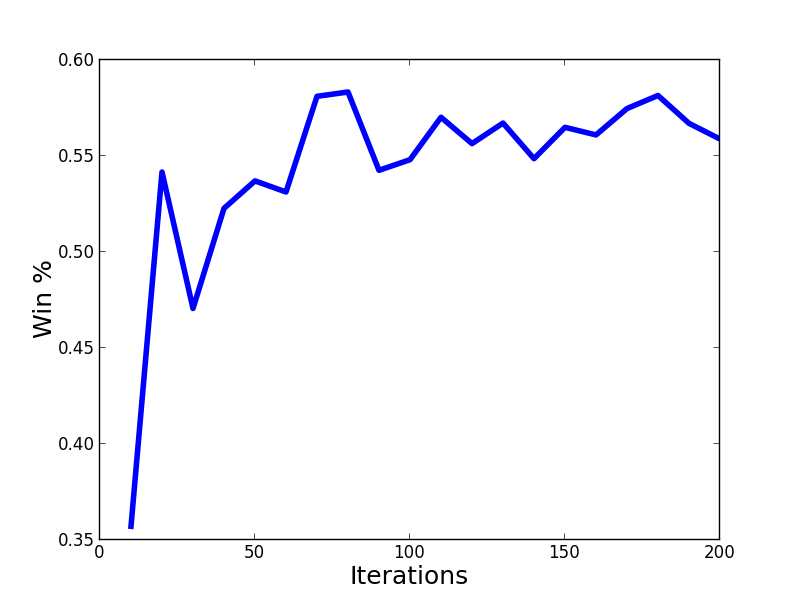
\includegraphics[scale=0.5]{figs/randvrand.png}
		\caption{Random Wins vs. Random}
		\label{fig:rand_v_rand}
\end{center}
\end{figure}
%%%%%%%%%
\subsection{Learner vs. Random Player}
\begin{table*}[hb!]
\centering
\begin{tabular}{| l | r | l | r | l |}
	\hline
 \textbf{Value} & \textbf{Wins}& \textbf{Losses}& \textbf{Total}& \textbf{Expected Win \%}\\
\hline
0& 148& 153& 301& 49.1749174917\\
1& 195& 66& 261& 74.5247148289\\
2& 22& 1& 23& 92.0\\
3& 9& 0& 9& 90.9090909091\\
4& 0& 0& 0& 50.0\\
5& 4& 0& 4& 83.3333333333\\
6& 2& 0& 2& 75.0\\
7& 0& 0& 0& 50.0\\
8& 0& 0& 0& 50.0\\
9& 0& 0& 0& 50.0\\
\hline
\end{tabular}
\caption{Expected Game Results, Learner vs. Random Player from Learner's Perspective}
\label{tab:learner_v_rand}
\end{table*}
\begin{figure}[ht!]
	\begin{center}
		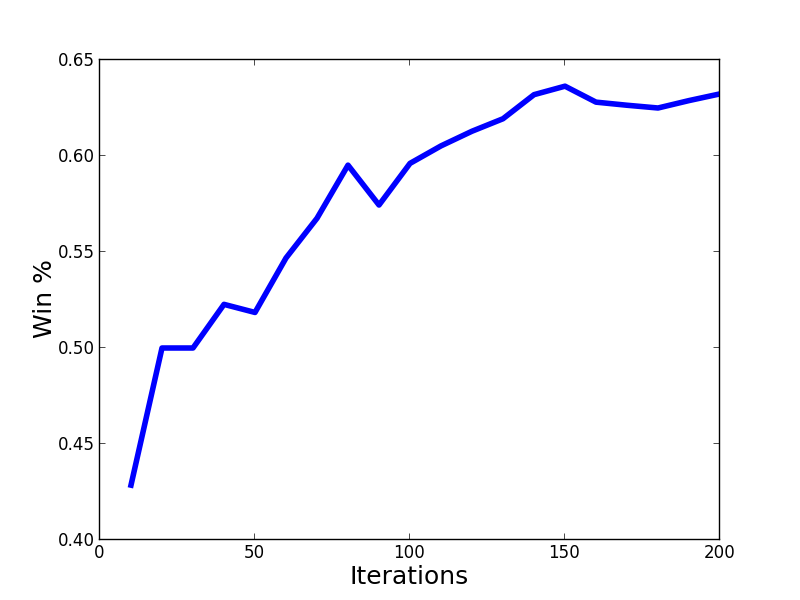
\includegraphics[scale=0.5]{figs/learnervrand.png}
		\caption{Learner Wins vs. Random}
		\label{fig:learner_v_rand}
\end{center}
\end{figure}

We pitted the learner against a random player to ascertain performance improvement in our learner over random actions. 
This performance improvement is evident in Table \ref{tab:learner_v_rand}. The learner, primed with the results from the random players, won 63\% of the time.  %TODO 

%%%%%%%%%%%
\subsection{Learner vs. Learner with background}
We pitted our learner against another instance of our learner, each with identical background information.
This background information included the body of results from the random players, as well as the body of results from the learner versus the random player. 
The winning percentages over a range of iterations is shown in Figure \ref{fig:learn_v_learn}.
\begin{table*}[hb!]
\centering
\begin{tabular}{| l | r | l | r | l |}
	\hline
 \textbf{Value} & \textbf{Wins}& \textbf{Losses}& \textbf{Total}& \textbf{Expected Win \%}\\
\hline
0& 26& 36& 62& 40.625\\
1& 35& 22& 57& 59.3220338983\\
2& 8& 0& 8& 80.0\\
3& 3& 0& 3& 60.0\\
4& 0& 0& 0& 0.0\\
5& 0& 0& 0& 0.0\\
6& 1& 0& 1& 33.3333333333\\
7& 0& 0& 0& 0.0\\
8& 0& 0& 0& 0.0\\
9& 0& 0& 0& 0.0\\
\hline
\end{tabular}
\caption{Expected Game Results, Learner1 vs. Learner2 from Learner1's perspective}
\label{tab:learner1_v_learner}
\end{table*}

\begin{table*}[hb!]
\centering
\begin{tabular}{| l | r | l | r | l |}
	\hline
 \textbf{Value} & \textbf{Wins}& \textbf{Losses}& \textbf{Total}& \textbf{Expected Win \%}\\
\hline
0& 24& 48& 72& 32.4324324324\\
1& 25& 24& 49& 49.0196078431\\
2& 5& 0& 5& 71.4285714286\\
3& 4& 1& 5& 57.1428571429\\
4& 0& 0& 0& 0.0\\
5& 0& 0& 0& 0.0\\
6& 0& 0& 0& 0.0\\
7& 0& 0& 0& 0.0\\
8& 0& 0& 0& 0.0\\
9& 0& 0& 0& 0.0\\
\hline
\end{tabular}
\caption{Expected Game Results, Learner1 vs. Learner2 from Learner2's perspective}
\label{tab:learner2_v_learner}
\end{table*}

\begin{figure}[ht!]
	\begin{center}
		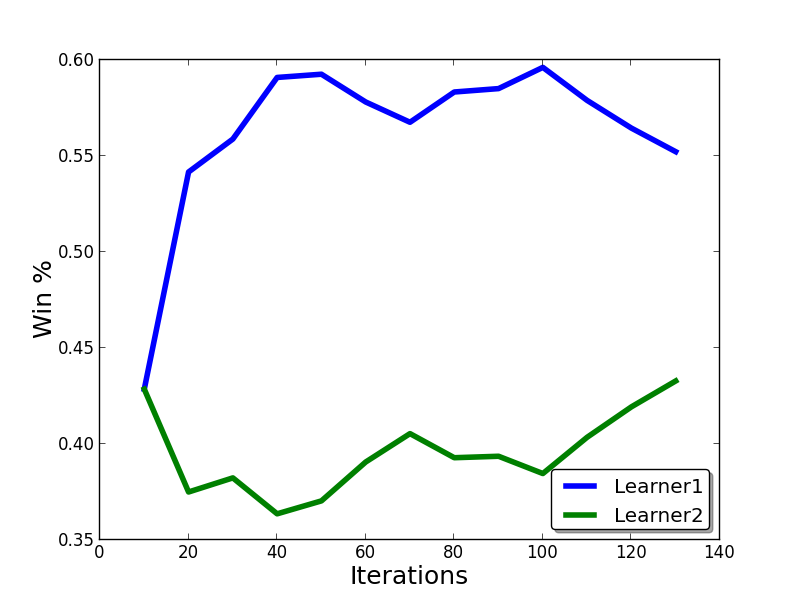
\includegraphics[scale=0.5]{figs/learnervlearner.png}
		\caption{Learner Wins vs. Learner}
		\label{fig:learn_v_learn}
\end{center}
\end{figure}

%%%%%%%%%%%
\subsection{Learner vs. Learner without background}

\subsection{Learner with background vs. Learner without background}
\section{Discussion}
%Discussion: discuss your results. What are the lessons of your experiments? What are the limitations of your approach? What would you suggest for future work in this direction?
\subsection{Results}
Results show
%Lessons include

\subsection{Limitations}   The value function currently only takes hand rank into account, not card value within rank. A hand of ``2 of Clubs, 3 of Hearts, 7 of Diamonds, Jack of Spades, Ace of Hearts'' is equivalent to ``2 of Hearts, 3 of Hearts, 7 of Diamonds, 8 of Spades, Jack of Hearts'' -- both are currently valued as ``high card'' hands, with no extra weight given to the ace-high hand. 
If these hands are played against each other, the ace-high hand will win and the jack-high hand will lose, but our learner does not take into account actual hand values seen in its predictive function.

\subsection{Future Work}
Future work includes incorporating wagers into \emph{All In}.  
Accounting for wagers is a much richer environment, and was outside the scope of this project.  
This would incorporate folding after the initial wager and deal, as well as tracking funds over a series of hands.
%TODO incorporate hands seen. 
% incorporate how many cards swapped -> wins

\section{Related Work}
There are many discussions of reinforcement learning and games, especially poker and its variants.
There does not seem to be any work on this particular variant of poker, five card draw.  

Erev et al.\ explore a variety of games, and show that their reinforcement model outperforms equilibrium predictions\cite{Erev98}.  

Dahl applies a reinforcement learning algorithm to two-layer Texas Hold'em Poker \cite{Dahl01}. 
This differs from our use of five card draw as a game, and changes the amount of information available about the other agent's status. 

Sweeney et al.\ explores the use of reinforcement learning to Texas Hold'em Poker\cite{Sweeney}.
This again differs from our use of five card draw as the game of choice.  
Wagering information and past actions of the opponent are taken into consideration in the described learning model.

\section{Conclusion}


\bibliographystyle{plain}
%\bibliography{}
\begin{thebibliography}{9}
\bibitem{korb99}
K.B. Korb, A.E. Nicholson and N. Jitnah,
 \emph{Bayesian Poker}. 
In Proc. of Uncertainty in Artificial Intelligence, pp. 343-350, 
Stockholm, Sweden, August, 1999.

%\bibitem{pokerdata}
%\emph{Poker Hand Data Set}
%http://archive.ics.uci.edu/ml/datasets/Poker+Hand

\bibitem{Sweeney}
Neill Sweeney, David Sinclair,
	\emph{Applying Reinforcement Learning to Poker}.
At Computer Poker Symposium, July, 2012.

\bibitem{Erev98}
Ido Erev and  Alvin E Roth, 
\emph{Predicting How People Play Games: Reinforcement Learning in Experimental Games with Unique, Mixed Strategy Equilibria}.
In American Economic Review, American Economic Association, vol. 88(4), pages 848-81, September, 1998.

\bibitem{Dahl01}
Fredrik A. Dahl, 
\emph{A Reinforcement Learning Algorithm Applied to Simplified Two-Player Texas Hold'em Poker}. 
In Proceedings of the 12th European Conference on Machine Learning (EMCL '01), Luc De Raedt and Peter A. Flach (Eds.). Springer-Verlag, London, UK, UK, 85-96, 2001.
\end{thebibliography}


\end{document}
